\section{Event Selection}
\label{sec:event_selection}

The event selection focuses on selecting events consistent with
$\bbbar\lephad$ or $\bbbar\hadhad$ final states. The selection
criteria applied to events are kept as loose as possible\todo{It could
  be looser...} given the limitations imposed by the trigger
selection. Distinguishing between signal and background events based
on object- and event-level observables is not the primary goal of the
event selection but rather of a multivariate analysis that will be
introduced at a later stage (in \Cref{sec:multivariate_analysis}). In
addition, suitable control and validation regions are defined for the
purpose of estimating background processes or validating background
estimates using data recorded by the ATLAS detector.

Events considered for further analysis are required to fulfil basic
quality criteria independent of the analysis channel:
\begin{itemize}
  % GRL + basic checks

  % eventInfoIn->errorState(xAOD::EventInfo::EventFlagSubDet::Tile) == xAOD::EventInfo::Error
  % Problems in tile calorimeter (``tile corrupted events''')
  %
  % eventInfoIn->errorState(xAOD::EventInfo::EventFlagSubDet::LAr) == xAOD::EventInfo::Error
  % LAr noise bursts
  %
  % eventInfoIn->errorState(xAOD::EventInfo::EventFlagSubDet::SCT) == xAOD::EventInfo::Error
  % SCT corrupted events (``recovery period after single event upset''')
  %
  % eventInfoIn->isEventFlagBitSet(xAOD::EventInfo::Core,18
  % Event info missing after TTC restart
\item All events are required to fulfil the data quality criteria by
  the ATLAS collaboration~\cite{DAPR-2018-01} requiring stable beams
  at the LHC and a fully operational detector.

  % Has vertex
\item The event is required to have a primary vertex.

  % No fake jets
  % DFCommonJets_eventClean_LooseBad
\item Events containing one or more jets that are classified as originating
  from non-collision backgrounds or calorimeter noise according to a
  \emph{loose} jet cleaning~\cite{ATLAS-CONF-2015-029} working point are
  rejected.
\end{itemize}

The search is divided into several analysis channels given by the
decay mode of the \taulepton pair and the type of trigger that
selected the event. The \lephad channel targets semi-leptonic decay
modes using single-lepton triggers (SLT) and lepton-plus-\tauhadvis
triggers (LTT). Each trigger category defines a corresponding
sub-channel, which are referred to as the \lephad SLT and \lephad LTT
channels. The \hadhad channel selects events with two \tauhadvis using
single-\tauhadvis triggers (STT) and di-\tauhadvis triggers
(DTT). While different types of triggers are used in the \hadhad
channel, the statistical analysis performed at a later stage will not
distinguish between events selected by STT and DTT, thus the \hadhad
final state is treated as a single analysis channel. In some cases,
for example for the background estimation, it will be required to
distinguish between both trigger categories. Cases where this applies
will be indicated explicitly.

Orthogonality between the \lephad and \hadhad channels is ensured by
the electron, muon, and \tauhadvis selections. In the \hadhad channel,
events are required to have exactly two \tauhadvis, vetoing events
with electrons or muons passing loose identification. Events in the
\lephad channels are required to have exactly one \tauhadvis and
exactly one electron or muon passing their respective loose
identification working point. Additionally, electrons (muons) are
required to pass the tight (medium) identification working point to
reduce backgrounds from jets being misidentified as electrons (muons).

Electrons, muons, and \tauhadvis have to be geometrically matched to
their corresponding objects at the HLT according to the trigger that
selected the event. Trigger-dependent transverse momentum thresholds
are applied to electrons, muons, and \tauhadvis to ensure that
triggers operate close to their trigger-efficiency plateau. The
thresholds applied in events selected by STT or SLT increased with
increasing instantaneous luminosity of the LHC during Run~2. In
contrast, lower \pT-thresholds on electrons, muons, and \tauhadvis
remained constant for DTT and LTT, trigger-rates instead being limited
by requiring additional jets and specific event topologies at the L1
trigger. The inclusion of the \lephad LTT channel allows to select
events with electrons or muons with transverse momenta below the SLT
\pT-threshold by requiring an additional \tauhadvis at
trigger-level. Orthogonality between the \lephad SLT and LTT channel
is ensured by only considering events with lepton \pT below the SLT
\pT-threshold for the LTT channel.

An overview of the signal region event selection for all search
channels is given in \Cref{tab:event_selection}. A more detailed
description of the \hadhad channel trigger selection will be given in
\Cref{sec:hadhad_trigger_selection}. Further selections applied at
event-level to define signal and control regions will be summarised in
\Cref{sec:sr_and_cr_selection}.

\begin{table}[htbp]
  \centering

  \caption{Summary of the signal region event selections for the
    \hadhad, \lephad SLT, and \lephad LTT channel. Trigger-dependent
    thresholds are applied to the transverse momentum of electrons,
    muons, and \tauhadvis. Where applicable, the range of these
    thresholds is listed.  Requirements on jets in the central region
    for the DTT or LTT category are trigger-dependent and thus not
    summarised in this table. For the \hadhad channel, the
    requirements resulting from the choice of triggers will be
    described in \Cref{sec:hadhad_trigger_selection}. Jets in the
    forward region are not used for event selection
    purposes. Requirements of the object selection introduced in
    \Cref{sec:object_reconstruction} are assumed to apply.}%
  \label{tab:event_selection}

  \resizebox{\textwidth}{!}{
    {
  \newcolumntype{C}[1]{>{\centering\let\newline\\\arraybackslash\hspace{0pt}}m{#1}}
  \small

  \begin{tabular}{C{0.225\textwidth}C{0.225\textwidth}C{0.225\textwidth}C{0.225\textwidth}}
    \toprule
    \multicolumn{2}{c}{\textbf{\hadhad channel}} & \multicolumn{2}{c}{\textbf{\lephad channels}} \\[0.5em]
    \textbf{STT} & \textbf{DTT} & \textbf{SLT} & \textbf{LTT} \\
    \midrule
    \multicolumn{4}{c}{\textbf{$e$ / $\mu$ selections}} \\
    \midrule
    \multicolumn{2}{c}{No loose $e$ or $\mu$} & \multicolumn{2}{c}{Exactly one loose $e$ or one loose $\mu$} \\[0.5em]
                                                 && \multicolumn{2}{c}{$e$ passes tight ID or} \\
                                                 && \multicolumn{2}{c}{$\mu$ passes medium ID and $|\eta| < 2.5$} \\[0.5em]
                                                 && $\pT(e) > 25\text{--}\SI{27}{\GeV}$ & $\pT(e) > \SI{18}{\GeV}$ \\
                                                 && $\pT(\mu) > 21\text{--}\SI{27}{\GeV}$ & $\pT(\mu) > \SI{15}{\GeV}$ \\[0.5em]
                                                 &&& Lepton \pT below SLT threshold \\
    \midrule
    \multicolumn{4}{c}{\textbf{\tauhadvis selections}} \\
    \midrule
    \multicolumn{2}{c}{Exactly two \tauhadvis} & \multicolumn{2}{c}{Exactly one \tauhadvis} \\[0.5em]
                                                 && \multicolumn{2}{c}{$|\eta| < 2.3$} \\[0.5em]
    $\pT > 100\text{--}180 \, (25)\,\si{\GeV}$ & $\pT > 40 \, (30)\,\si{\GeV}$ & & $\pT > \SI{30}{\GeV}$ \\
    \midrule
    \multicolumn{4}{c}{\textbf{Central jet selections ($|\eta| < 2.5$)}} \\
    \midrule
    \multicolumn{4}{c}{$\geq 2$ jets}\\[0.5em]
    $\geq 1$ jet with $\pT > \SI{45}{\GeV}$ & Trigger-dependent & $\geq 1$ jet with $\pT > \SI{45}{\GeV}$ & Trigger-dependent \\
    \midrule
    \multicolumn{4}{c}{\textbf{Event-level selections}} \\
    \midrule
    \multicolumn{4}{c}{Event is selected by a trigger and trigger requirements are fulfilled} \\[0.25em]
    \multicolumn{4}{c}{Exactly 2 $b$-tagged jets} \\[0.25em]
    \multicolumn{4}{c}{Opposite sign electric charge between \tauhadvis and $e$ / $\mu$ / \tauhadvis} \\[0.25em]
    \multicolumn{4}{c}{$\mMMC > \SI{60}{\GeV}$} \\[0.25em]
                                                 && \multicolumn{2}{c}{$\mBB < \SI{150}{\GeV}$} \\
    \bottomrule
  \end{tabular}
}

%%% Local Variables:
%%% mode: latex
%%% TeX-master: "../phd_thesis"
%%% End:

  }
\end{table}


\subsection{Trigger selection in the \hadhad channel}%
\label{sec:trigger}%
\label{sec:hadhad_trigger_selection}

The triggers used to select events of interest for the \hadhad channel
are summarised in \Cref{tab:triggers_hadhad}. The choice of triggers
depends on the data-taking period and will be motivated in the
following. Reconstruction or selections applied at the level of the
full event reconstruction will be qualified by \emph{offline} (e.g.\
offline reconstruction, offline selection/requirements) to distinguish
them from trigger-level (\emph{online}) reconstruction or selections.

\begin{sidewaystable}[p]
  \centering

  \caption{List of single- and di-\tauhadvis triggers used in the
    \hadhad channel. The trigger naming conventions of the ATLAS
    collaboration are used and summarised in the following. The
    \pT-thresholds on \tauhadvis at the HLT are denoted by
    \texttt{tauX}, where \texttt{X} is the threshold in
    \si{\GeV}. Three different \tauhadvis HLT chains are used, the
    differences between them are explained in the main body. \ET and
    isolation requirements for \tauhadvis at the L1 trigger are
    denoted by \texttt{XTAUY}(\texttt{I}/\texttt{IM}) with \texttt{Y}
    referring to the \ET-threshold in \si{\GeV},
    \texttt{I}/\texttt{IM} the isolation requirements, and \texttt{X}
    the number of \tauhadvis fulfilling these criteria. Jets at the L1
    trigger are similarly denoted by \texttt{XJY}(\texttt{.0ETA23}),
    where \texttt{Y} refers to the jet \ET-threshold in \si{\GeV}, the
    suffix \texttt{.0ETA23} referring to a requirement of
    $|\eta| < 2.3$ on jets, and \texttt{X} the number of jets
    fulfilling these conditions. Unless a trigger is based on the L1
    topological trigger system~\cite{TRIG-2019-02} (L1Topo), here
    chains using the \texttt{DR-TAU20ITAU12I-J25} seed, no
    disambiguation between objects at L1 is performed such that one
    \texttt{TAU20IM} also ensures at least one count of
    \texttt{TAU12IM}, \texttt{J20}, and \texttt{J12}. For chains based
    on L1Topo, disambiguation is performed and additionally \tauhadvis
    at L1 are required to fulfil
    $\Delta R(\tau_0^{\text{L1}}, \tau_1^{\text{L1}}) \leq 2.8$.
    Requirements on \tauhadvis and jets from offline event
    reconstruction (offline requirements) are imposed. These
    requirements are specified in terms of the leading or sub-leading
    \tauhadvis ($\tau_0$ or $\tau_1$) or the leading or sub-leading
    central jet ($\text{j}_0$ or $\text{j}_1$). For all events
    selected by DTT, \tauhadvis have to fulfil
    $\pT(\tau_0) > \SI{40}{\GeV}$ and $\pT(\tau_1) >
    \SI{30}{\GeV}$. The data-taking periods where triggers were used
    are given in the last column.}%
  \label{tab:triggers_hadhad}

  \resizebox{\textwidth}{!}{
    \begin{tabular}{lllll}
  \toprule
  \textbf{HLT chain} & \textbf{} & \textbf{L1 trigger} & \textbf{Offline event selection} & \textbf{Period} \\
  \midrule
  \multicolumn{5}{l}{Single-\tauhadvis triggers} \\
  \midrule
  \texttt{tau80} & \texttt{medium1\_tracktwo} & \texttt{TAU60} & $\pT(\tau_0) > \SI{100}{\GeV}$ & 15--16 A \\
  \texttt{tau125} & \texttt{medium1\_tracktwo} & \texttt{TAU60} & $\pT(\tau_0) > \SI{140}{\GeV}$ & 16 B--16 D3\\
  \texttt{tau160} & \texttt{medium1\_tracktwo} & \texttt{TAU60} & $\pT(\tau_0) > \SI{180}{\GeV}$ & 16 D4--17 B4\\
  \texttt{tau160} & \texttt{medium1\_tracktwo} & \texttt{TAU100} & $\pT(\tau_0) > \SI{180}{\GeV}$ & 17 B5--17 end\\
  \texttt{tau160} & \texttt{medium1\_tracktwoEF} & \texttt{TAU100} & $\pT(\tau_0) > \SI{180}{\GeV}$ & 18-- \\
  \texttt{tau160} & \texttt{mediumRNN\_tracktwoMVA} & \texttt{TAU100} & $\pT(\tau_0) > \SI{180}{\GeV}$ & 18 K-- \\
  \midrule
  \multicolumn{5}{l}{Di-\tauhadvis triggers} \\
  \midrule
  \texttt{tau35} + \texttt{tau25} & \texttt{medium1\_tracktwo} & \texttt{TAU20IM\_2TAU12IM} & $\pT(\text{j}_0) > \SI{80}{\GeV}$ & 15--15 end \\
  \texttt{tau35} + \texttt{tau25} & \texttt{medium1\_tracktwo} & \texttt{TAU20IM\_2TAU12IM\_J25\_2J20\_3J12} & $\pT(\text{j}_0) > \SI{80}{\GeV}$ & 16--17 B4 \\
  \texttt{tau35} + \texttt{tau25} & \texttt{medium1\_tracktwo} & \texttt{TAU20IM\_2TAU12IM\_4J12} & $\pT(\text{j}_1) > \SI{45}{\GeV}$ & 17--17 end \\
  \texttt{tau35} + \texttt{tau25} & \texttt{medium1\_tracktwo} & \texttt{DR-TAU20ITAU12I-J25} & $\pT(\text{j}_0) > \SI{80}{\GeV}$, $\Delta R(\tau_0, \tau_1) < 2.5$ & 17 B5--17 end \\
  \texttt{tau35} + \texttt{tau25} & \texttt{medium1\_tracktwoEF} & \texttt{TAU20IM\_2TAU12IM\_4J12.0ETA23} & $\pT(\text{j}_1) > \SI{45}{\GeV}$ & 18-- \\
  \texttt{tau35} + \texttt{tau25} & \texttt{medium1\_tracktwoEF} & \texttt{DR-TAU20ITAU12I-J25} & $\pT(\text{j}_0) > \SI{80}{\GeV}$, $\Delta R(\tau_0, \tau_1) < 2.5$ & 18-- \\
  \texttt{tau35} + \texttt{tau25} & \texttt{mediumRNN\_tracktwoMVA} & \texttt{TAU20IM\_2TAU12IM\_4J12.0ETA23} & $\pT(\text{j}_1) > \SI{45}{\GeV}$ & 18 K-- \\
  \texttt{tau35} + \texttt{tau25} & \texttt{mediumRNN\_tracktwoMVA} & \texttt{DR-TAU20ITAU12I-J25} & $\pT(\text{j}_0) > \SI{80}{\GeV}$, $\Delta R(\tau_0, \tau_1) < 2.5$ & 18 K-- \\
  \bottomrule
\end{tabular}

%%% Local Variables:
%%% mode: latex
%%% TeX-master: "../phd_thesis"
%%% End:

  }
\end{sidewaystable}

As Run~2 of the LHC progressed, several improvements were made to the
HLT algorithms for \tauhadvis triggers. In total three different
\tauhadvis HLT chains are used:
\begin{description}

\item[\texttt{medium1\_tracktwo}] This chain is the primary HLT chain
  for \tauhadvis triggers from
  2015--2017~\cite{ATL-DAQ-PUB-2016-001,ATL-DAQ-PUB-2017-001,ATL-DAQ-PUB-2018-002}. A
  brief summary, derived from Ref.~\cite{ATLAS-CONF-2017-061}, is
  given here.

  First, a purely calorimeter-based reconstruction of the \tauhadvis
  candidate is performed in the region of interest (ROI) provided by
  the L1 trigger. The topo-cluster algorithm is applied to cells of
  energy in the calorimeters, the resulting clusters calibrated using
  a scheme accounting for the different response of the calorimeter to
  $e^\pm$/$\gamma$ and hadrons. The energy of \tauhadvis candidates is
  determined from clusters in a core region ($\Delta R < 0.2$) around
  the barycentre of cluster energies in the ROI, subsequently applying
  a \tauhadvis-specific calibration which is a function of \tauhadvis
  candidate \pT, $\eta$, and pile-up conditions. HLT thresholds on the
  transverse momentum of \tauhadvis candidates are applied after these
  steps.

  Second, a two-stage tracking
  approach~\cite{TRIG-2016-01,ATLAS-CONF-2017-061} using \emph{fast
    tracking}, instead of the more time-consuming \emph{precision
    tracking}, is employed. As a first stage, fast tracking is
  performed in a narrow region surrounding the \tauhadvis ROI centre
  but extended over a large section of the beamline. The \pT-leading
  track resulting from the first stage is used to narrow down the
  search space along the beamline by only considering tracks within
  $|\Delta z| < \SI{10}{\milli\metre}$ of this track, allowing to
  widen the search region around the ROI centre for the second
  stage. After the second stage of fast tracking, multiplicities of
  core ($\Delta R < 0.2$) and isolation tracks
  ($0.2 < \Delta R < 0.4$) are defined. Track multiplicity
  requirements are applied by selecting \tauhadvis candidates at the
  HLT with one to three tracks in the core and at most one track in
  the isolation region.

  As a final step, a \tauhadvis selection similar to the offline
  \tauhadvis selection is performed. The tracks resulting from the
  two-stage tracking are used as seeds for precision tracking. The
  precision tracks are then used to calculate discriminating variables
  used for \tauid. Finally, a BDT-based \tauid algorithm, similar to
  its counterpart from the offline \tauhadvis reconstruction, is
  applied requiring \tauhadvis to pass a medium efficiency working
  point.\footnote{The working points of the trigger-level \tauid do
    not correspond to the efficiencies of the \tauid of the offline
    reconstruction. The medium working point at trigger-level applies
    less stringent selections than the loose working point of offline
    \tauid.}

\item[\texttt{medium1\_tracktwoEF}]
  % The precision tracks are also called EF tracks, while fast tracks
  % are called FTF tracks.
  This chain was introduced for data-taking in
  2018~\cite{ATL-DAQ-PUB-2019-001} and differs from the previous one
  by delaying the track multiplicity selections to a later stage of
  the HLT chain. Instead of counting tracks from the two-stage fast
  track finding, the track multiplicities are defined using precision
  tracks. This change circumvented a reduction in efficiency for
  3-prong \tauhadvis in high pile-up conditions due to the fast track
  finding being more susceptible to fake
  tracks~\cite{ATL-DAQ-PUB-2019-001}.

\item[\texttt{mediumRNN\_tracktwoMVA}] This chain started operation in
  period K of 2018 data-taking~\cite{ATL-DAQ-PUB-2019-001}. The
  integrated luminosity from period K to the end of Run~2 corresponds
  to about \SI{37}{\per\femto\barn}. Several changes were implemented
  on top of the previous chain.

  First, the \tauhadvis energy calibrations as part of the
  calorimeter-based \tauhadvis reconstruction are replaced by
  multivariate methods, namely Boosted Regression Trees. Second, the
  trigger-level \tauid is replaced by an identification algorithm
  based on RNN, adopting the approach taken for offline \tauid,
  offering improved rejection of \tauhadvis originating from quark- or
  gluon-jets at the HLT. The improved background rejection allows to
  relax the track multiplicity cuts from 1--3 precision tracks to 0--3
  precision tracks in the core region. Allowing \tauhadvis candidates
  without precision tracks in the core region recovers cases where the
  fast track finding does not yield good quality seeds for the
  precision tracking.  After the offline event reconstruction, a
  fraction of these events can be correctly reconstructed, thus
  improving the selection efficiency of the trigger.
\end{description}
From period K in 2018 onwards, the use of a logical \emph{or} between
the \texttt{medium1\_tracktwoEF} and \texttt{mediumRNN\_tracktwoMVA}
chains is recommended, calibrations for this combination being
centrally provided by the ATLAS collaboration. This recommendation is
followed in the trigger selection employed in this search.

In the \hadhad channel, single- and di-\tauhadvis triggers are used to
select events of interest. When an event fulfills both the STT and DTT
criteria, the criteria being discussed in the following, precedence is
given to STT.

The STT used during Run~2 data-taking had changing \pT-thresholds
applied to \tauhadvis at trigger-level. At the HLT, these threshold
ranged from \SI{80}{\GeV} up to \SI{160}{\GeV}. To ensure that the
triggers operate close to their trigger-efficiency plateau, it is
required that one \tauhadvis from the offline reconstruction can be
geometrically matched to the \tauhadvis at the HLT ($\Delta R < 0.2$)
and that the offline \tauhadvis transverse momentum exceeds the HLT
threshold by \SIrange{15}{20}{\GeV}. The exact requirements on
\tauhadvis are listed in~\Cref{tab:triggers_hadhad}.

At the HLT, the requirements imposed on \tauhadvis transverse momenta
by DTT remain unchanged throughout Run~2 of the LHC, requiring the
leading and sub-leading \tauhadvis to exceed transverse momenta of
\SI{35}{\GeV} and \SI{25}{\GeV}, respectively. To ensure that the
triggers are close to fully efficient, two \tauhadvis from offline
reconstruction are required to be geometrically matched to \tauhadvis
at the HLT and exceed the corresponding HLT threshold by at least
\SI{5}{\GeV}. The primary limitations of di-\tauhadvis triggers arise
at the L1 trigger, necessitating changes in the L1 seeds used for
these triggers as the instantaneous luminosity of the LHC increased
during Run~2.

In 2015, the DTT had no additional requirements beyond two isolated
\tauhadvis at the L1 trigger. However, an offline requirement on the
\pT-leading jet in the central region is imposed, requiring
$\pT > \SI{80}{\GeV}$. This selection is not strictly necessary and is
applied to harmonise the selection with the one applied for triggers
used for the remainder of Run~2.\footnote{The integrated luminosity
  collected in 2015 is small (\SI{3.2}{\per\femto\barn}) compared to
  the full Run~2 $pp$-collision dataset thus motivating the use of a
  cut that is tighter than necessary in favour of harmonising the
  selection between data-taking periods.}

In 2016, requirements of additional jets were added to L1 seeds of DTT
to limit the rate at which events were accepted. Three jets were
required, two of which overlapping with \tauhadvis ROIs since no
disambiguation is performed between \tauhadvis and jets at the L1
trigger.\footnote{At the L1 trigger, a \tauhadvis candidate with
  transverse energy of $\ET^\tau$ is also reconstructed as a jet ROI
  with $\ET^{\text{jet}} \geq \ET^\tau$.}  The \ET-thresholds applied
to the three jets are \SI{25}{\GeV}, \SI{20}{\GeV}, and \SI{12}{\GeV},
the two lowest thresholds ensured to be fulfilled due to the
\tauhadvis requirements at the L1 trigger (cf.\
\Cref{tab:triggers_hadhad}). The \ET-threshold applied to the jet not
overlapping with a \tauhadvis ROI can be lower than \SI{25}{\GeV}
provided a \tauhadvis candidate exists that is also reconstructed as a
jet with $\ET > \SI{25}{\GeV}$. However, an offline requirement of
$\pT > \SI{80}{\GeV}$ is still applied to the leading jet in the
central region, which corresponds to the trigger efficiency plateau of
the L1 jet trigger with a threshold of $\ET > \SI{25}{\GeV}$.

In 2017, DTT based on two new L1 seeds were introduced, one
specifically developed for this search
(\texttt{TAU20IM\_2TAU12IM\_4J12}), and one a continuation of the DTT
used in 2016 with additional requirements at L1 to cope with the
increase in instantaneous luminosity
(\texttt{DR-TAU20ITAU12I-J25}). Both trigger chains are used in this
search, the trigger being chosen depending on the phase space selected
in the search. If the transverse momentum of the sub-leading central
jet from the offline event reconstruction exceeds \SI{45}{\GeV} the
trigger chain based on the \texttt{TAU20IM\_2TAU12IM\_4J12} seed is
used. This chain requires two additional jets with
$\ET > \SI{12}{\GeV}$ at L1, the offline requirement on the
sub-leading jet \pT ensuring that the trigger operates close to its
efficiency plateau. This type of DTT will be referred to as
\FourJTwelve. If the condition for the \FourJTwelve trigger is not
fulfilled but the event has a leading central jet from offline
reconstruction with $\pT > \SI{80}{\GeV}$ and $\dRtautau < 2.5$ then
the DTT with the \texttt{DR-TAU20ITAU12I-J25} seed is considered. This
trigger is based on the L1 topological trigger
system~\cite{TRIG-2019-02} that allows to disambiguate between jet and
\tauhadvis ROIs and to apply other topological requirements at the L1
trigger. As a result of the disambiguation, the jet requirement at L1
is stricter compared to the DTT used in 2016. Additionally, only
events with a $\Delta R \leq \num{2.8}$ between \tauhadvis ROIs at L1
are considered. The phase space where this trigger is employed is
chosen such that the L1 requirements are fully efficient. Due to the
use of the L1 topological trigger system, this type of trigger will be
referred to as \LOneTopo in the following.

The \FourJTwelve trigger was introduced to enhance the acceptance of
signals from scalar resonances with low mass and the acceptance of
non-resonant \HH production with low invariant masses of the
\HH-system (\mHH). The \LOneTopo trigger limits the acceptance of
signals in this phase space due to the high \pT-threshold on the
leading jet and the \dRtautau requirement. For resonances with masses
beyond \SI{325}{\GeV} and SM \HH production, which has a sufficiently
hard \mHH spectrum, the signal acceptance improvement of using both
\FourJTwelve and \LOneTopo triggers is negligible over just using the
\LOneTopo trigger.

In 2018, new \tauhadvis HLT algorithms were introduced, updating the
existing \LOneTopo- and \FourJTwelve-based trigger chains. Changes
were made to the selections applied by the \FourJTwelve L1 seed for
DTT, requiring at least four jets with $\ET > \SI{12}{\GeV}$ and
$|\eta| < 2.3$ instead. This change introduced a mismatch in the
pseudorapidity selection for \tauhadvis ($|\eta| < 2.5$) and jet ROIs
($|\eta| < 2.3$) at the L1 trigger, such that the L1 jet multiplicity
requirement was not specified as intended. This was problematic when
one or more \tauhadvis at L1 are close to the boundary of the
acceptance in pseudorapidity such that they do not count towards the
number of jets in $|\eta| < 2.3$. Moreover, the pseudorapdity
requirement on jets does not align with the offline event selection
where jets can be \btagged up to $|\eta| < 2.5$. This mismatch caused
an inefficiency in the trigger selection for signal processes,
cancelling the efficiency improvements obtained at the HLT from to the
$\texttt{medium1\_tracktwoEF}$ chains, such that the trigger
efficiency remained at the level of the \FourJTwelve trigger used in
2017. The relative reduction in trigger efficiency for signal
processes compared to the \FourJTwelve trigger without the
$|\eta| < 2.3$ requirement is approximately \SI{5}{\percent}. This
issue is resolved in the trigger menu to be used for Run~3 of the LHC
by extending the pseudorapidity range for the jets at L1.

A flowchart summarising the trigger selection is shown
in~\Cref{fig:trigger_selection_flowchart}. Two features of the trigger
selection are not explicitly illustrated in the figure. First, the
\LOneTopo trigger only started operation with period B5 in 2017 while
the \FourJTwelve was available from the start of 2017 data-taking. In
the intermittent period where \LOneTopo was not available, the
unprescaled \tauhadvis trigger chain based on
\texttt{TAU20IM\_2TAU12IM\_J25\_2J20\_3J12} is used instead, however,
also applying the $\dRtautau < 2.5$ selection necessary for
\LOneTopo. Second, for three runs in 2017 the L1 topological trigger
system was disabled due to problems with the trigger firmware. For
these runs the DTT chain based on
\texttt{TAU20IM\_2TAU12IM\_J25\_2J20\_3J12} was used as a backup. This
chain was almost unprescaled during these runs, losing about
\SI{60}{\per\pico\barn} of integrated luminosity in the \LOneTopo
category as a result of the prescale.

\begin{figure}[htbp]
  \centering

  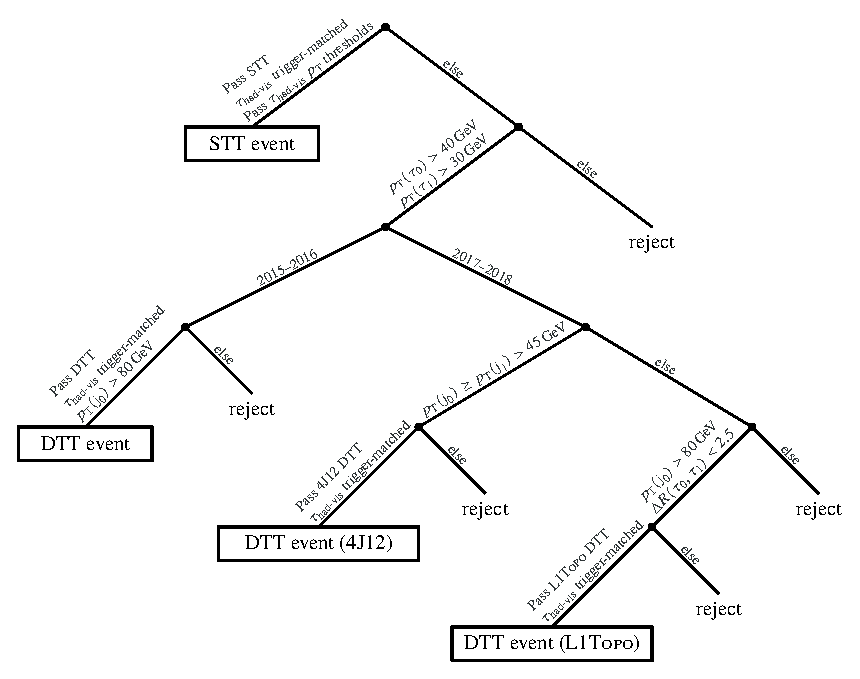
\includegraphics[width=\textwidth]{selection/trigger_flowchart}

  \caption{Flowchart of the \hadhad channel trigger selection. The
    leading and sub-leading \tauhadvis candidate (jet) from the
    offline event reconstruction are abbreviated as $\tau_0$ and
    $\tau_1$ ($\text{j}_0$ and $\text{j}_1$), respectively.}%
  \label{fig:trigger_selection_flowchart}
\end{figure}

After applying the

Some trigger efficiency plot would be nice???

STT selects only few events, predominately targeting regions of high resonance mass / high mHH.

Possible plots to add:
J25 turn-on???
dRtautau for L1Topo turn-on???
J12 turn-on???

\subsection{Signal and control region event selection}%
\label{sec:sr_and_cr_selection}

% Make a note here that the basic object multiplicities need to be fulfilled?
The signal regions are defined for all events passing the trigger
selection and the associated cuts on \tauhadvis and jets from the
offline event selection. Only regions with exactly two \btagged jets
(2 $b$-tag regions) are considered as signal regions, regions with
fewer \btagged jets being largely dominated by backgrounds do not
contribute significantly to the signal sensitivity. Regions with fewer
than two \btagged jet (0 and 1 $b$-tag regions) are used as
control/validation regions for the background estimation instead.

The electric charge of the electron, muon, or \tauhadvis candidate has
to be reconstructed with opposite-sign (OS) with respect to the charge
of the other \tauhadvis candidate in the event. Events from processes
producing \tauleptons such as the signal processes, \Zjets,
$H \to \tautau$, \ttbar are expected to be reconstructed with OS
charges. Events with same-sign (SS) electric charge of the
$H \to \tautau$ candidate objects are predominantely originating from
events containing \tauhadvis mimicked by quark- or gluon-initiated
jets. Therefore, the SS region is used in the \hadhad channel for the
estimation of the multi-jet background.

All events considered in this search are required to successfully pass
the di-$\tau$ mass reconstruction using the MMC. Additionally,
Drell-Yan processes producing \taulepton pairs with low invariant mass
are rejected by requiring $\mMMC > \SI{60}{\GeV}$.

In the \lephad channels, the signal regions only consider events with
$\mBB < \SI{150}{\GeV}$. The purpose of this selection is to allow the
definition of a \ttbar control region depleted of signal events by
inverting by inverting the cut on \mBB. This region is used for
measurements related to the \faketauhadvis background estimation in
the \lephad and \hadhad channels.

The expected event yields after the signal region selection of all
three channels is summarised in~\Cref{tab:smhh_prefit_yields}. The
bulk of events entering the signal regions are from top quark
backgrounds, \Zjets, and backgrounds where a quark- or gluon-initiated
jet mimics the signature of a \tauhadvis (\jettotauhadvis).

\begin{table}[htbp]
  \centering

  \caption{Expected event yields in all three signal regions prior to
    the fit. The yields are shown including all statistical and
    systematic uncertainties. The \faketauhadvis background estimation
    technique employed in the \lephad channels does not distinguish
    between different sources of \faketauhadvis (the majority is
    expected to originate from \ttbar).  The category ``other
    backgrounds'' combines minor contributions from
    $Z \to \tautau + (bl,cl,ll)$, $Z \to e^{+}e^{-}$,
    $Z \to \mu^{+}\mu^{-}$, \Wjets, diboson and $\ttbar V$. The
    background estimation and systematic uncertainties will be
    discussed in detail
    in~\Cref{sec:background_estimation,sec:uncertainties}. The SM \HH
    event yields are given for a signal strength according to the SM
    expectation.}%
  \label{tab:smhh_prefit_yields}%
  \label{tab:hadhad_presel_yields}

  \resizebox{\textwidth}{!}{
    \begin{tabular}{l
  @{\hskip 20pt}
  S[table-format=4.3(4)]
  @{\hskip 20pt}
  S[table-format=6.3(4)]
  @{\hskip 20pt}
  S[table-format=4.4(5)]}
  \toprule
  & \multicolumn{3}{c}{Signal region event yield} \\
  \cmidrule{2-4}
  Process                              & {\hadhad}      & {\lephad SLT}  & {\lephad LTT} \\
  \midrule
  SM \HH (ggF)                         & 5.4 +- 1.1     & 5.9 +- 1.2     & 1.42 +- 0.29 \\
  SM \HH (VBF)                         & 0.167 +- 0.022 & 0.200 +- 0.027 & 0.0547 +- 0.0066 \\
  SM \HH (ggF + VBF)                   & 5.6 +- 1.1     & 6.1 +- 1.2     & 1.47 +- 0.29 \\
  \midrule
  Top quark                            & 3850 +- 330    & 65300 +- 5600  & 4400 +- 460 \\
  $Z \to \tautau + (bb,bc,cc)$         & 1200 +- 210    & 1210 +- 130    & 406 +- 67 \\
  Single Higgs boson                   & 74 +- 15       & 154 +- 20      & 24.4 +- 5.0 \\
  Jet $\to \faketauhadvis$ (combined)  & {--}           & 33900 +- 6500  & 1750 +- 510 \\
  Jet $\to \faketauhadvis$ (multi-jet) & 1350 +- 150    & {--}           & {--} \\
  Jet $\to \faketauhadvis$ (\ttbar)    & 2490 +- 330    & {--}           & {--} \\
  Other backgrounds                    & 228 +- 42      & 1090 +- 210    & 119 +- 21 \\
  \midrule
  Total background                     & 9200 +- 640    & 101700 +- 8600 & 6700 +- 700 \\
  \midrule
  Observed data                        & 8380           & 98456          & 6351 \\
  \bottomrule
\end{tabular}

%%% Local Variables:
%%% mode: latex
%%% TeX-master: "../phd_thesis"
%%% End:

  }
\end{table}

% Maybe say that the analysis is statistically limited thus the changes
% to generally looser object identification criteria for taus and
% b-jets.

The acceptance times efficiency, \AccTimesEff, of the signal region
selection for the SM \HH signal is summarised
in~\Cref{tab:nonres_acc_times_eff}. Compared to the previously
published result in this channel~\cite{HIGG-2016-16-witherratum}, this
search selects SM \HH with improvements in the \AccTimesEff by a
factor exceeding 2 (1.5) for the \hadhad channel (\lephad
channels). This increase is an effect of improved \tauhadvis
reconstruction techniques and loosened object selection requirements
for \tauhadvis and \btagged jets compared to the previously published
result. The reason for using a loosened object selection is
two-fold. First, the \tauhadvis identification and $b$-tagging
algorithms were significantly improved for analyses of the
\SI{139}{\per\femto\barn} $pp$-collision dataset, yielding reduced
mistag rates at working points with tagging efficiencies similar to
the algorithms that were previously used. This allows the use of
looser object selection criteria while maintaining background rates
similar to the taggers used previously. Second, when using further
selections exploiting the distinct features of Higgs boson pair
production to isolate events of interest (e.g.\ using multivariate
methods), then the sensitivity of this search is expected to be
limited by statistical uncertainties. A looser object selection can
thus serve to improve the signal sensitivity, provided the increase in
rate of backgrounds arising from events with mistagged objects remains
under control.

\begin{table}[htbp]
  \centering

  \caption{Acceptance times efficiency of the SM \HH signal for the
    signal region selection of all three channels. The acceptance
    times efficiency is given with respect to all generated
    $pp \to \HH \to \bbbar\hadhad$ ($pp \to \HH \to \bbbar\lephad$)
    events for the \hadhad channel (\lephad channels). A comparison
    with the signal acceptance of the previous iteration of the
    analysis is given in the last row, the values taken from
    Ref.~\cite{HIGG-2016-16-witherratum}. $\dagger$:~The SM \HH
    acceptance times efficiency is given for the combination of
    \lephad SLT and LTT channel.}%
  \label{tab:nonres_acc_times_eff}

  \begin{tabular}{lSSS}
  \toprule
  & \multicolumn{3}{c}{Acceptance $\times$ Efficiency / \si{\percent}} \\
  \cmidrule{2-4}
  Process &\hadhad & \lephad SLT & \lephad LTT \\
  \midrule
  SM \HH (\ggF)       & 4.1 & 4.1 & 0.99 \\
  SM \HH (VBF)        & 2.3 & 2.5 & 0.68 \\
  SM \HH (\ggF + VBF) & 4.0 & 4.0 & 0.97 \\
  \midrule
  SM \HH (\ggF, early Run~2 search~\cite{HIGG-2016-16-witherratum}) & 1.9 & \multicolumn{2}{c}{3.2$^\dagger$} \\
  \bottomrule
\end{tabular}

% hadhad:
% ggF: 4.08
% VBF: 2.27
% ggF+VBF: 3.99

% lephad SLT:
% ggF: 4.08
% VBF: 2.50
% ggF+VBF: 4.00

% lephad LTT:
% ggF: 0.99
% VBF: 0.68
% ggF+VBF: 0.97

%%% Local Variables:
%%% mode: latex
%%% TeX-master: "../phd_thesis"
%%% End:

\end{table}

The majority of the increase in the SM \HH \AccTimesEff of the signal
region selections with respect to Ref.~\cite{HIGG-2016-16-witherratum}
can be explained by changes in \tauhadvis reconstruction,
identification and $b$-tagging:
\begin{description}

\item[Improvements in track selection for \tauhadvis] The introduction
  of a multivariate method for \tauhadvis track selection lead to an
  improvement in the \tauhadvis reconstruction efficiency. The new
  method, introduced in Ref.~\cite{duschinger}, supersedes a cut-based
  track selection method, leading to a relative improvement in 1-prong
  (3-prong) \tauhadvis reconstruction efficiency of \SI{6}{\percent}
  (\SI{10}{\percent}).

\item[Improvements in \tauhadvis identification]
  The increased background rejection of the RNN \tauid compared to the
  BDT ID allowed to switch from the medium working point that was used
  previously to the loose working point while maintaining similar
  background rates. This lead to a relative improvement in \tauhadvis
  tagging efficiency of \SI{13}{\percent} (\SI{25}{\percent}) for
  1-prong (3-prong) \tauhadvis.

  The likelihood-based electron veto algorithm was replaced by an
  algorithm based on a BDT discriminant.


  relative increase in tagging
  efficiency of \SIrange{4}{5}{\percent} for 1-prong \tauhadvis. No
  electron veto is applied for 3-prong \tauhadvis candidates.

\item[Improvements in $b$-tagging]

  The increased light and charm jet rejection of the \textsc{DL1r}
  tagger~\cite{ATL-PHYS-PUB-2017-013}.

  The previous analysis used \textsc{MV2c10}
  tagger~\cite{ATL-PHYS-PUB-2016-012} with target tagging efficiency
  for true $b$-jets in \ttbar of \SI{70}{\percent}.

  \SI{10}{\percent} relative improvement
\end{description}
The object-level efficiency improvements compound due to the
requirement of 2 $b$-tagged jets and two (one) \tauhadvis in the
\hadhad (\lephad) signal regions explaining the large improvement in
\AccTimesEff for SM \HH with respect to the previous
search.\todo{Should make a note of the backgrounds here.}

The acceptance times efficiency, \AccTimesEff, of the SM \HH
production and resonant production of \HH is shown
in~\Cref{tab:nonres_acc_times_eff} and
\Cref{fig:signal_acceptance_resonant}, respectively.

Signal acceptance non-res HH (ggf / VBF)

Signal acceptance improvement compared to previous analysis.

Two-fold improvement with respect to the previous analysis. Reasons:
- Switch from 70\% efficiency MV2c10 tagger to 77\% DL1r tagger
- Improved \tauhadvis track counting leading to 6\% relative efficiency improvement for 1-prong \tauhadvis reconstruction and \SI{10}{\percent} 3-prong \tauhadvis reconstruction
- Improved electron-Veto algorithm improving 1-prong \tauhadvis efficiency from ca.\ \SI{92}{\percent} to \SI{96}{\percent}
- Switch from medium BDT ID (75 / 60) to loose RNN ID (85 / 75)

Accounting for these efficiency improvements leads to a two-fold improvement in signal acceptance in the \hadhad channel.

\todo[inline]{SR selection (not really applicable -- maybe talk about PNN)??? Anti-Tau CR}

\todo[inline]{Observables used to reduce backgrounds: dRTauTau, dRBB, mtautau,
  mbb, mHH}










\begin{figure}[htbp]
  \centering

  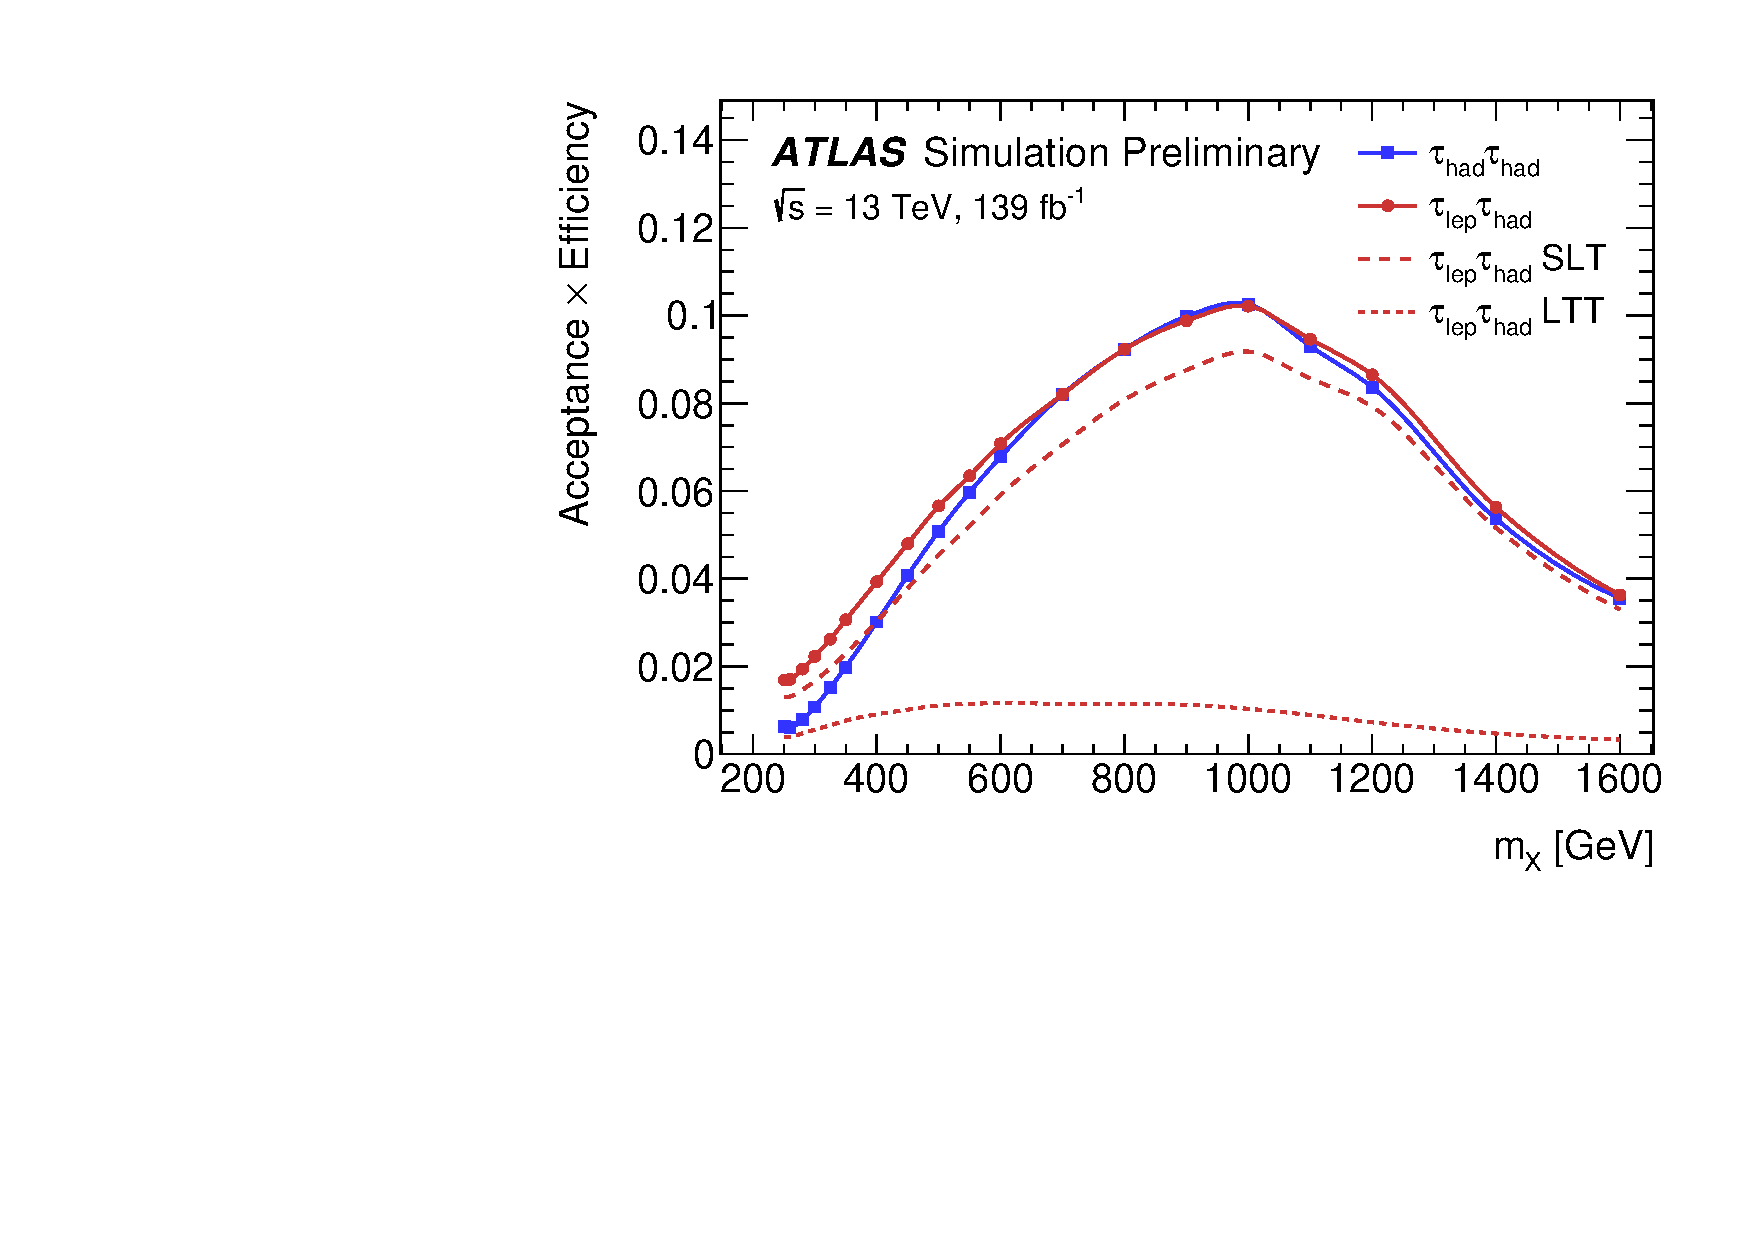
\includegraphics[width=0.6\textwidth]{selection/acceptance_resonant}

  \caption{Acceptance times efficiency for scalar resonances of narrow
    width decaying into \HH in the signal regions of all three
    analysis channels and the combination of the \lephad SLT and LTT
    channels. The acceptance times efficiency is given with respect to
    all generated $X \to \HH \to \bbbar\hadhad$
    ($X \to \HH \to \bbbar\lephad$) events for the \hadhad channel
    (\lephad channels). The figure is taken from
    Ref.~\cite{ATLAS-CONF-2021-030}.}%
  \label{fig:signal_acceptance_resonant}

  \todo[inline]{Update to paper version}
\end{figure}

Control region definitions briefly listed with references to the
chapters where they are used:
\begin{description}

\item[$Z$+$bb$ control region ($Z \to e^+e^-$/$\mu^+\mu^-$)] Z+bb
  control region in $e^+e^-$ and $\mu^+\mu^-$ final state with two
  \btagged jets.

\item[Top control region (\lephad)] $\mBB > \SI{150}{\GeV}$

\item[Anti-ID and same-sign control regions (\hadhad)] Multi-jet (1
  $b$-tag) or multi-jet and \ttbar (2 $b$-tag)

\item[]

\end{description}


The SR selection is as follows:
\begin{itemize}
\item Exactly two reconstructed \tauhadvis passing \textit{loose} identification
  (RNN)

\item Unit electric charge of \tauhadvis candidate with opposite sign as
  reconstructed from the tracks associated to the \tauhadvis candidates

\item Two or more jets

\item Exactly two \btagged jets with the \SI{77}{\percent} working point of the
  DL1r tagger

\item No reconstructed and identified electrons and muons in the event

\item Passing the trigger selection described in \cref{sec:trigger}

\item The \tauhadvis are geometrically matched to objects that fired either the
  STT or the DTT trigger.

\item \mMMC > \SI{60}{\GeV}

\item At least one \bjet with \pT > \SI{45}{\GeV} \todo{Can we drop this?}
\end{itemize}


Orthogonality between the L1Topo and the 4J12 DTT is ensured by offline cuts on
\tauhadvis and jet \pT:
\begin{itemize}
\item STT events: \tauhadvis are required to pass a trigger-dependent \pT
  threshold as described in \cref{sec:trigger}. STT events are prioritised over
  DTT events.

\item DTT events in 2015-2016: The leading jet is required to have \pT >
  \SI{80}{\GeV} due to the additional jet requirement (J25) at L1 in 2016. This
  ensures that the L1 trigger is close to its efficiency plateau, minimizing the
  impact of a mismatch in trigger efficiency in data / MC.

\item DTT events in 2017-2018: Are categorised into two categories depending on
  the triggers to be checked:\todo{Chris: need to check treatment of non-L1Topo
    trigger at the beginning of 2017}
  \begin{itemize}
  \item If leading and subleading jet $\pT > \SI{45}{\GeV}$: Event is considered a
    4J12 event. This cut ensures that the additional jet requirement at L1 (J12)
    is fulfilled.
  \item Else if leading jet $\pT > \SI{80}{\GeV}$ and $\dRtautau \leq 2.5$:
    Event is considered a L1Topo event. The jet \pT and \dRtautau cut ensure
    that the additional J25 and \dRtautau requirement at L1 are fulfilled.
  \end{itemize}
\end{itemize}


%%% Local Variables:
%%% mode: latex
%%% TeX-master: "../../phd_thesis"
%%% End:
